\RequirePackage{luatex85}

\documentclass[tikz]{standalone}

\usepackage[siunitx]{circuitikz}

\usetikzlibrary{calc}

\tikzset{
  neuron/.style={
    % The shape:
    circle,
    % The size:
    minimum size=6mm,
    % The border:
    very thick,
    draw=blue!50!black!50,
        % The filling:
    top color=white,
    bottom color=blue!50!black!20, % and something else at the bottom
    % Font
    font=\itshape,
    % padding around node
    % outer sep=2mm
  }
}


\begin{document}

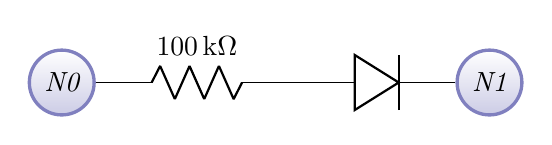
\begin{tikzpicture}

  \node [neuron] (n0) at (0, 0) {N0};

  \draw (n0.east) to [R, l=100<\kilo\ohm>] (3, 0) coordinate (junction);

  \draw (junction) to [diode] (5, 0) node (n1) [right, neuron] {N1};

\end{tikzpicture}

\end{document}
